\section{Additional Treatment Effects Tables \& Effect Plots} \label{sec:appxa}

\subsection{Full set of Treatment Effects for Housing Prices}

The full set of treatment effects provided in Table \ref{tab:median_sale_amount_full} support Table \ref{tab:median_sale_amount} which provides treatment effects for the housing price outcome variable in the main body of the paper. These treatment effects are estimated using a regression model that controls for various factors.

\begin{table}[htbp]
    \centering
    \caption{Full set of estimates - Median Housing Price}
    \label{tab:median_sale_amount_full}
    \begin{tabular}{p{3cm}cccc}
        \hline
        \textbf{Year relative to vote} & \textbf{Estimate} & \textbf{Standard error} & \textbf{p-value} & \textbf{Confidence interval} \\
        \hline
        $t - 3$  & 3,468   & 7,465  & 0.642  & [-11,164, 18,099] \\
        $t - 2$  & -1,703  & 6,617  & 0.797  & [-14,673, 11,267] \\
        $t - 1$  & 1,784   & 6,950  & 0.797  & [-11,838, 15,407] \\
        $t + 1$ & -6,197  & 9,662  & 0.521  & [-25,134, 12,741] \\
        $t + 2$ & -17,059 & 9,518  & 0.073  & [-35,715, 1,597] \\
        $t + 3$ & -9,823  & 8,244  & 0.233  & [-25,981, 6,335] \\
        $t + 4$ & -19,535 & 9,289  & 0.035  & [-37,741, -1,329] \\
        $t + 5$ & -21,531 & 9,147  & 0.019  & [-39,459, -3,604] \\
        $t + 6$ & -16,994 & 7,558  & 0.025  & [-31,809, -2,180] \\
        $t + 7$ & -16,991 & 7,357  & 0.023  & [-31,111, -2,272] \\
        $t + 8$ & -23,323 & 9,449  & 0.014  & [-41,842, -4,803] \\
        $t + 9$ & -30,620 & 9,586  & 0.001  & [-49,408, -11,833] \\
        $t + 10$ & -16,411 & 9,342  & 0.079  & [-34,721, 1,898] \\
        \hline
    \end{tabular}
    \begin{tablenotes}
        \small
        \item Supplements Table \ref{tab:median_sale_amount} in text. Full set of treatment effect estimates of renewing road tax levies relative to cutting road tax levies from 3 years before the vote to 10 years after the vote. Covariates from Table \ref{tab:variable_means_sd} used in all regressions. Outcome is median house price in constant 2010 U.S. dollars. Unit of observation is the city-year. A treatment effect of -\$19,535 means that four years after the vote, cities that vote to cut road taxes and its associated spending have houses that sell for \$19,535 less than cities that vote to renew road taxes and spending.
    \end{tablenotes}
\end{table}

% \begin{figure}[htbp]
%     \centering
%     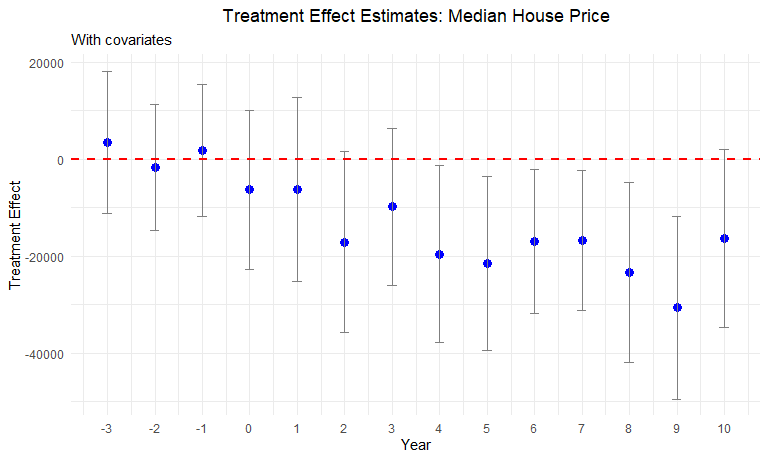
\includegraphics[width=\textwidth,keepaspectratio]{images/tes_gs.png}
%     \caption{Event Study - Median Housing Price}
%     \label{fig:tes_gs_app}
% \end{figure}

\clearpage


% \subsection{Outcome vs Running variable plots for years after Treatment}

\clearpage

\section{Additional Robustness Tests} \label{sec:appxb}

\subsection{Covariate Discontinuity Tests \& Smoothness Plots}

\begin{table}[!h]
    \centering
    \caption{Covariate Discontinuity Test Results}
    \label{tab:covariate_discontinuity}
    \begin{tabular}{p{2cm}cccc}
        \hline
        Variable & Estimate & Standard error & p-value & Confidence interval \\
        \hline
        Population                           & -388      & 1,094   & 0.722  & [-2,532, 1,755] \\
        Poverty Rate                         & 0.017     & 0.014   & 0.234  & [-0.011, 0.045] \\
        \% with Kids                         & -0.007    & 0.012   & 0.539  & [-0.030, 0.015] \\
        \% Households with Children under 18 & 0.0001    & 0.007   & 0.981  & [-0.014, 0.014] \\
        \% Less than High School Education   & -0.004    & 0.020   & 0.834  & [-0.043, 0.035] \\
        \% Some College Education            & -0.012    & 0.011   & 0.274  & [-0.034, 0.009] \\
        \% Unemployment Rate                 & -0.002    & 0.006   & 0.733  & [-0.013, 0.009] \\
        \% Renters                           & -0.005    & 0.015   & 0.754  & [-0.035, 0.025] \\
        \% White                             & -0.007    & 0.011   & 0.499  & [-0.028, 0.014] \\
        \% Black                             & -0.004    & 0.009   & 0.685  & [-0.021, 0.014] \\
        \% Married                           & -0.013    & 0.015   & 0.374  & [-0.042, 0.016] \\
        \% Separated                         & 0.001     & 0.002   & 0.485  & [-0.002, 0.004] \\
        \hline
    \end{tabular}
    \begin{tablenotes}
        \small
        \item Estimates indicate the treatment effect of failing to renew a road maintenance tax levy on each covariate considered during our study. Confidence intervals are presented in square brackets.
    \end{tablenotes}
\end{table}

% \subsection{Covariate Smoothness Plots}

\begin{figure}[ht]
    \centering
    \begin{minipage}[b]{0.40\textwidth}
        \centering
        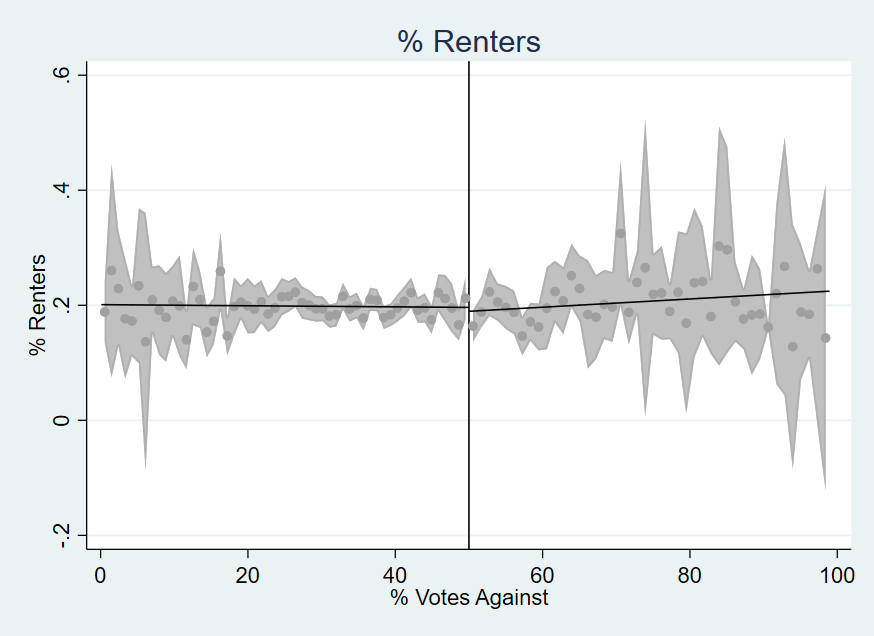
\includegraphics[width=\textwidth,keepaspectratio]{images/cov_smoothness_pctrent.png}
        \caption*{Pct Rent}
        \label{fig:pctrent_sm}
    \end{minipage}
    \hfill
    \begin{minipage}[b]{0.40\textwidth}
        \centering
        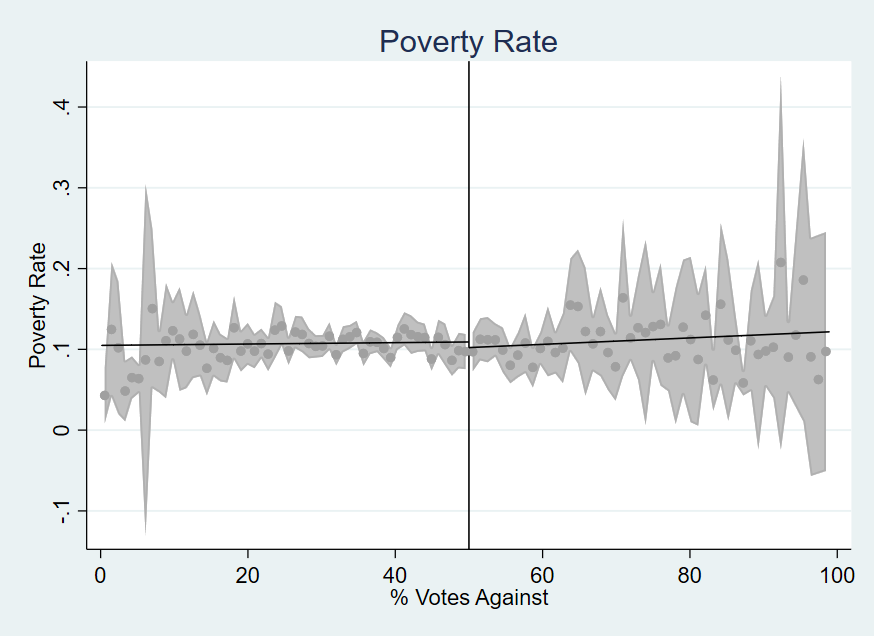
\includegraphics[width=\textwidth,keepaspectratio]{images/cov_smoothness_poverty.png}
        \caption*{Poverty Rate}
        \label{fig:poverty_sm}
    \end{minipage}
    
    % \vspace{1em}
    
    \begin{minipage}[b]{0.40\textwidth}
        \centering
        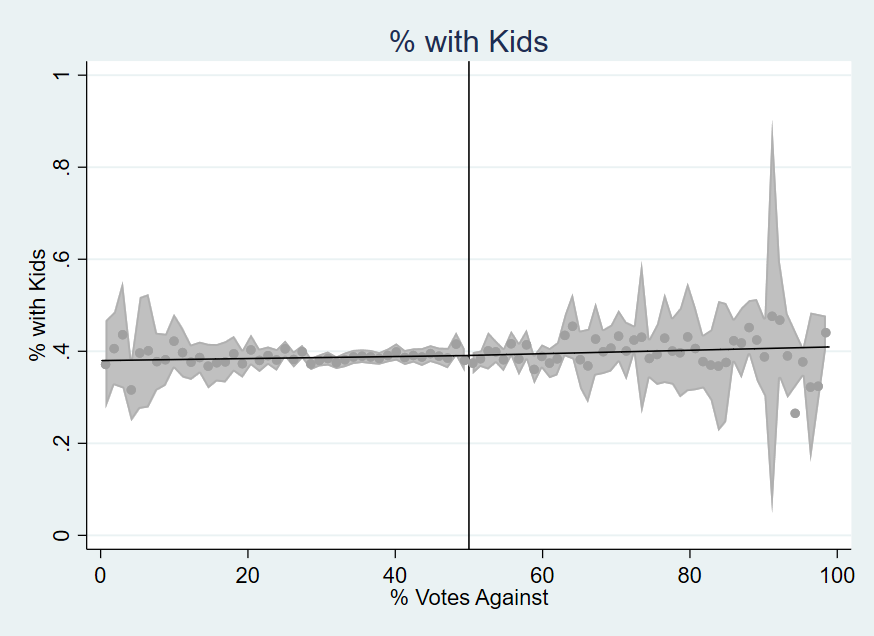
\includegraphics[width=\textwidth,keepaspectratio]{images/cov_smoothness_pctwithkids.png}
        \caption*{Pct With Kids}
        \label{fig:pct_with_kids_sm}
    \end{minipage}
    \hfill
    \begin{minipage}[b]{0.40\textwidth}
        \centering
        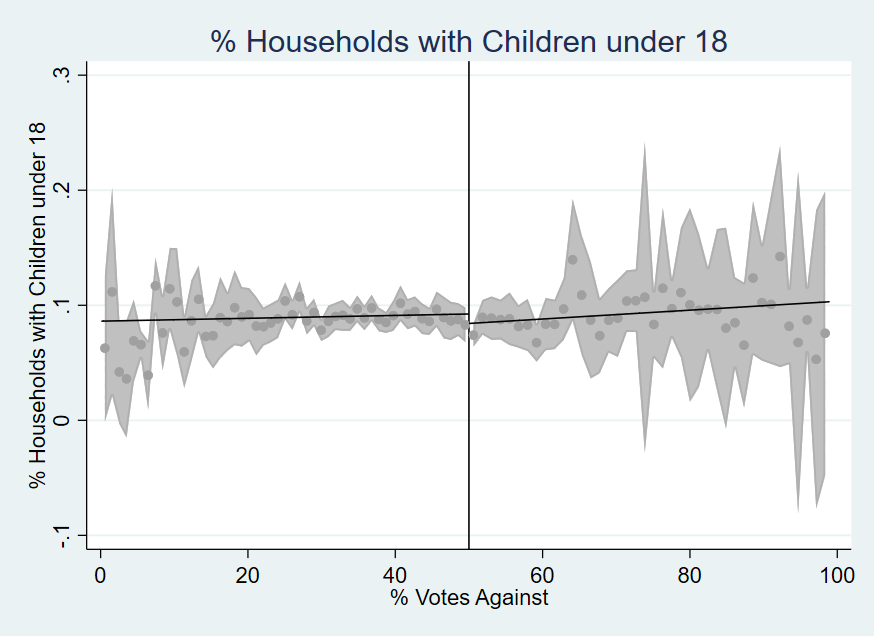
\includegraphics[width=\textwidth,keepaspectratio]{images/cov_smoothness_pctsinparhhld.png}
        \caption*{Pct Single Parent Hhld}
        \label{fig:pctsinparhhld_sm}
    \end{minipage}
    
    % \vspace{1em}
    
    \begin{minipage}[b]{0.40\textwidth}
        \centering
        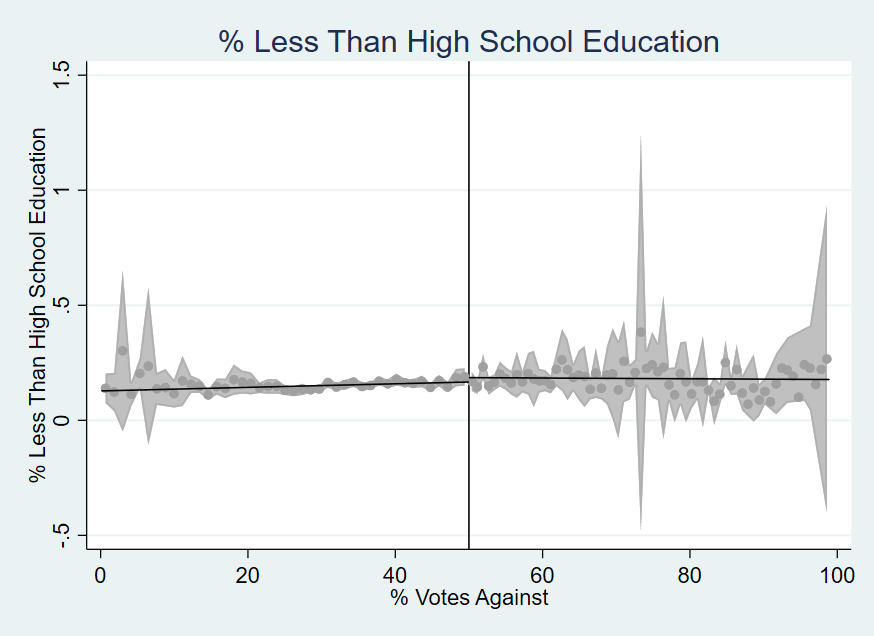
\includegraphics[width=\textwidth,keepaspectratio]{images/cov_smoothness_pctlesshs.png}
        \caption*{Pct Less than HS}
        \label{fig:pctlesshs_sm}
    \end{minipage}
    \hfill
    \begin{minipage}[b]{0.40\textwidth}
        \centering
        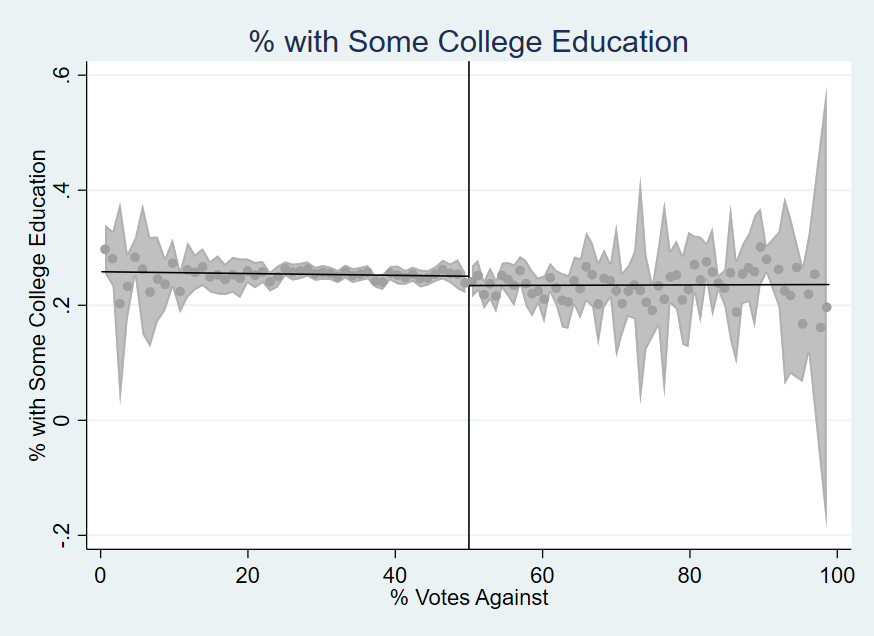
\includegraphics[width=\textwidth,keepaspectratio]{images/cov_smoothness_pctsomecoll.png}
        \caption*{Pct Some College}
        \label{fig:pctsomecoll_sm}
    \end{minipage}
    
    % \vspace{1em}
    
    \begin{minipage}[b]{0.40\textwidth}
        \centering
        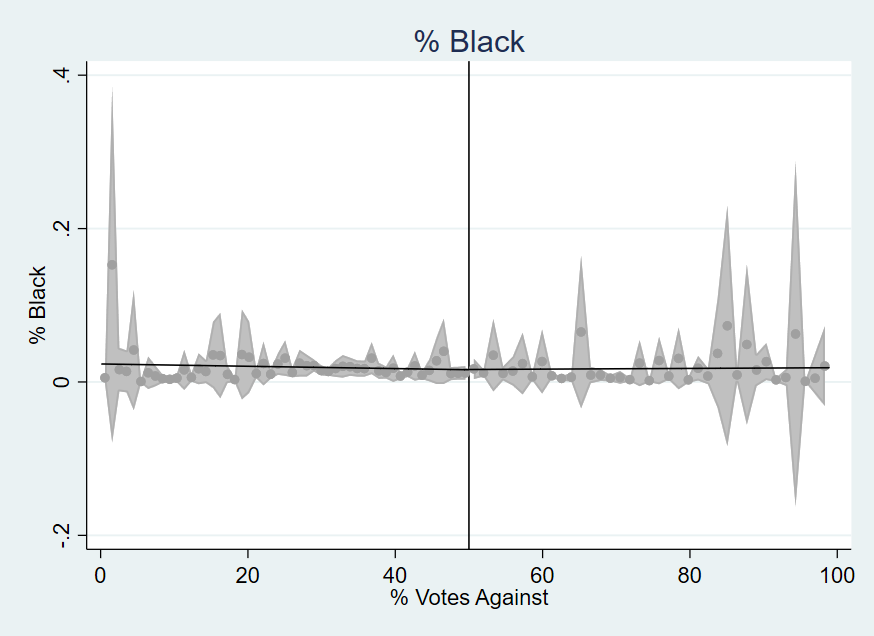
\includegraphics[width=\textwidth,keepaspectratio]{images/cov_smoothness_pctblack.png}
        \caption*{Pct Black}
        \label{fig:black_sm}
    \end{minipage}
    \hfill
    \begin{minipage}[b]{0.40\textwidth}
        \centering
        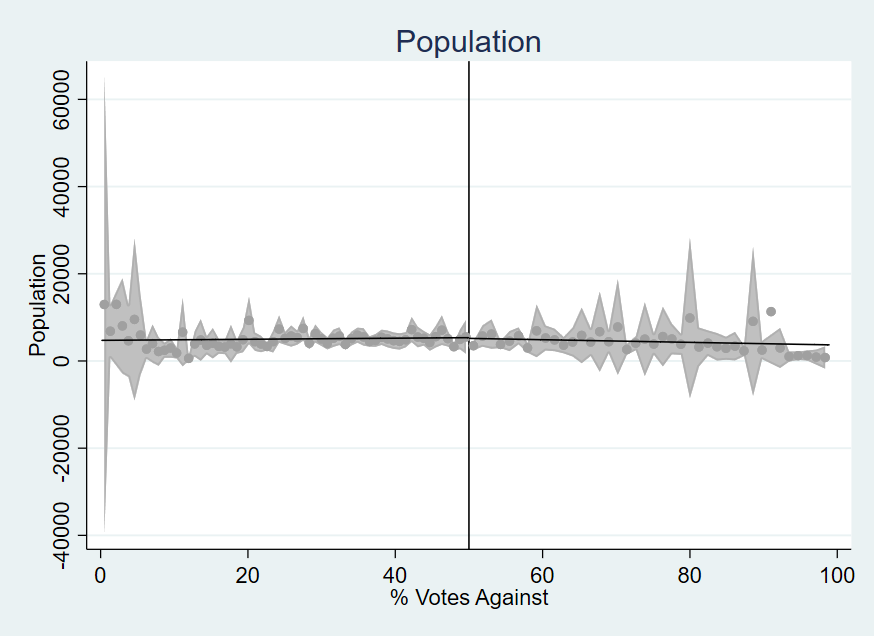
\includegraphics[width=\textwidth,keepaspectratio]{images/cov_smoothness_pop.png}
        \caption*{Population}
        \label{fig:pop_sm}
    \end{minipage}
    
    \caption{Covariate Discontinuity Plots - Part 1}
    \label{fig:rd_cov_smoothness_1}
\end{figure}

\begin{figure}[ht]
    \centering
    \begin{minipage}[b]{0.40\textwidth}
        \centering
        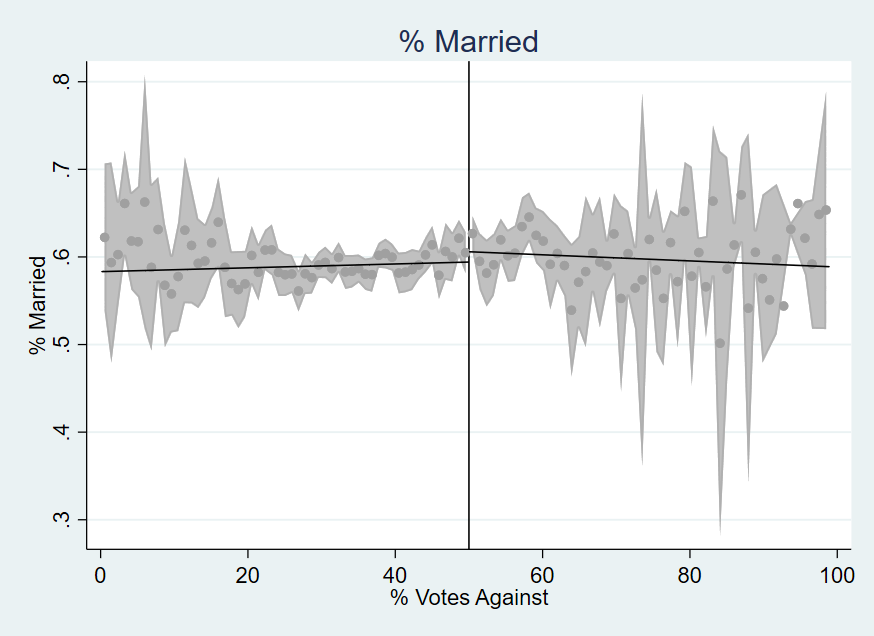
\includegraphics[width=\textwidth,keepaspectratio]{images/cov_smoothness_pctmarried.png}
        \caption*{Pct Married}
        \label{fig:pctmarried_sm}
    \end{minipage}
    \hfill
    \begin{minipage}[b]{0.40\textwidth}
        \centering
        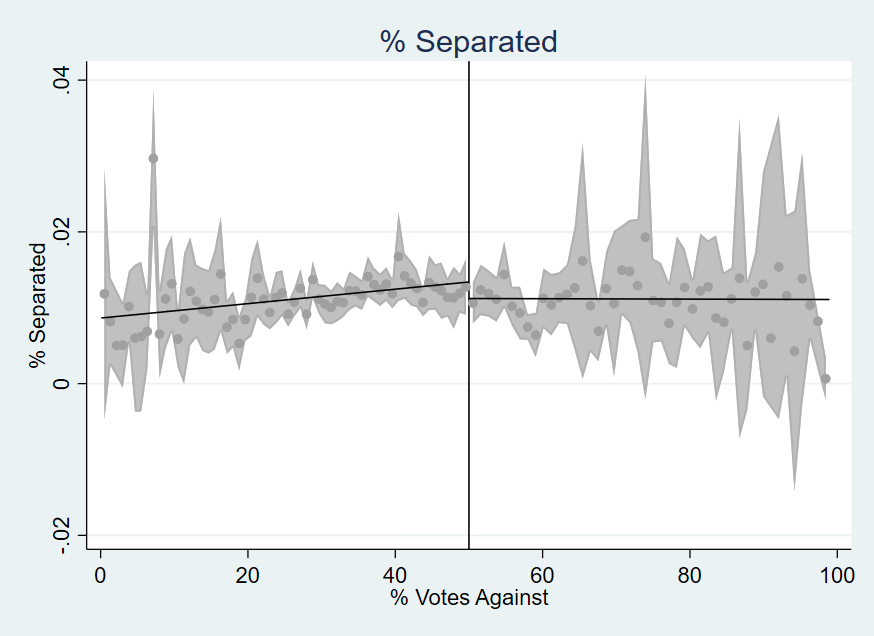
\includegraphics[width=\textwidth,keepaspectratio]{images/cov_smoothness_pctseparated.png}
        \caption*{Pct Separated}
        \label{fig:pctseparated_sm}
    \end{minipage}
    
    \vspace{1em}
    
    \begin{minipage}[b]{0.40\textwidth}
        \centering
        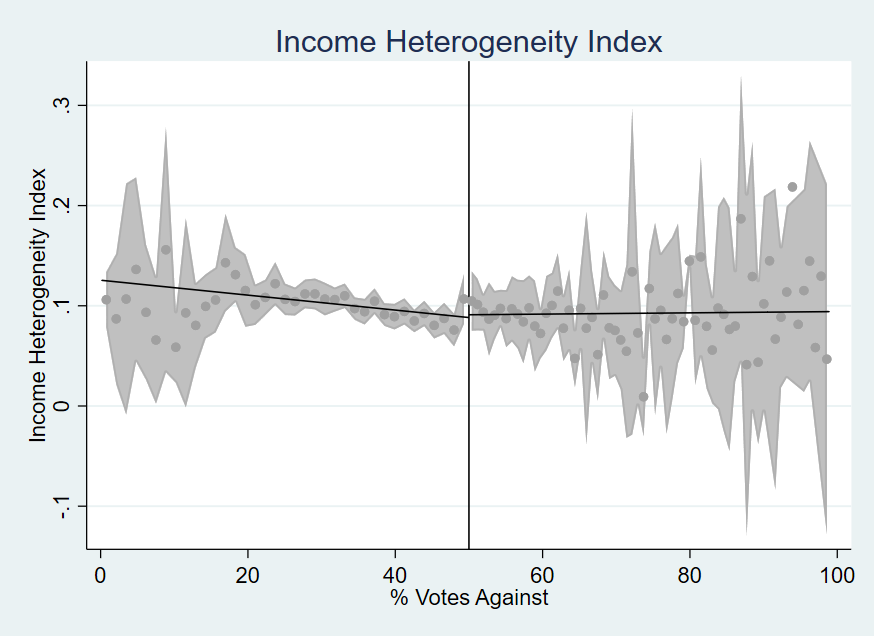
\includegraphics[width=\textwidth,keepaspectratio]{images/cov_smoothness_incherfindahl.png}
        \caption*{Income Herfindahl Index}
        \label{fig:incherfindahl_sm}
    \end{minipage}
    \hfill
    \begin{minipage}[b]{0.40\textwidth}
        \centering
        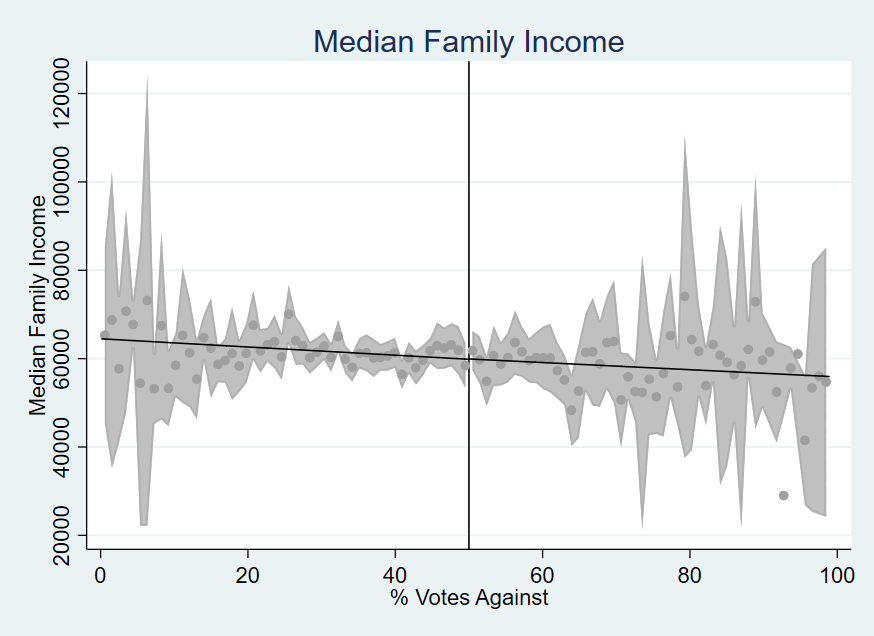
\includegraphics[width=\textwidth,keepaspectratio]{images/cov_smoothness_medfamy.png}
        \caption*{Median Family Income}
        \label{fig:medfamy_sm}
    \end{minipage}
    
    \vspace{1em}
    
    \begin{minipage}[b]{0.40\textwidth}
        \centering
        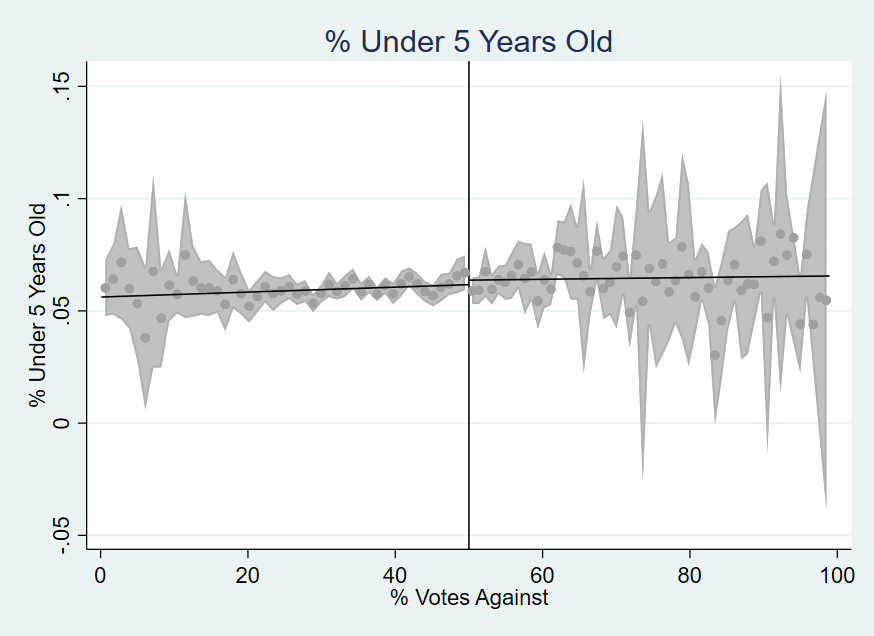
\includegraphics[width=\textwidth,keepaspectratio]{images/cov_smoothness_pctlt5.png}
        \caption*{Pct Less than 5}
        \label{fig:pctlt5_sm}
    \end{minipage}
    \hfill
    \begin{minipage}[b]{0.40\textwidth}
        \centering
        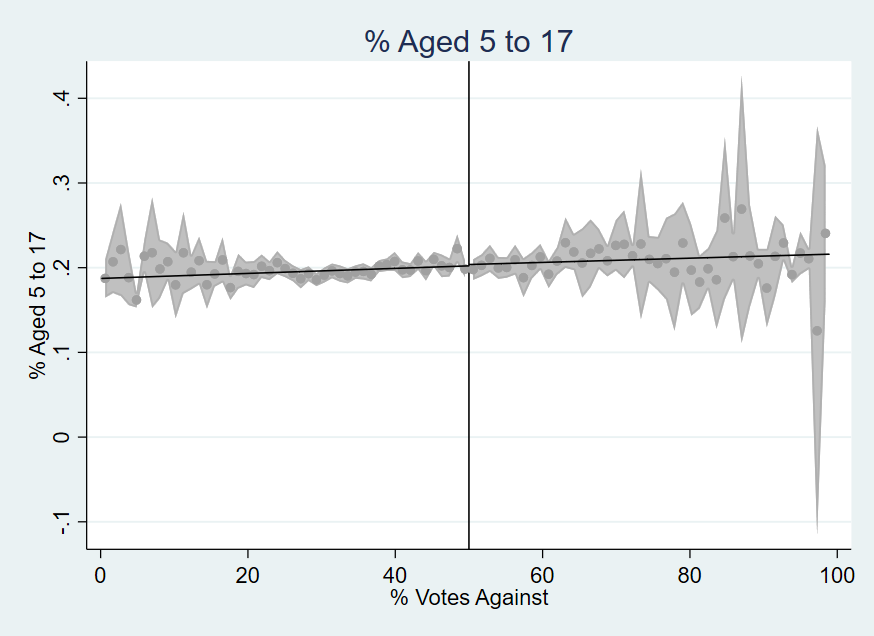
\includegraphics[width=\textwidth,keepaspectratio]{images/cov_smoothness_pct5to17.png}
        \caption*{Pct 5 to 17}
        \label{fig:pct5to17_sm}
    \end{minipage}
    
    \vspace{1em}
    
    \begin{minipage}[b]{0.40\textwidth}
        \centering
        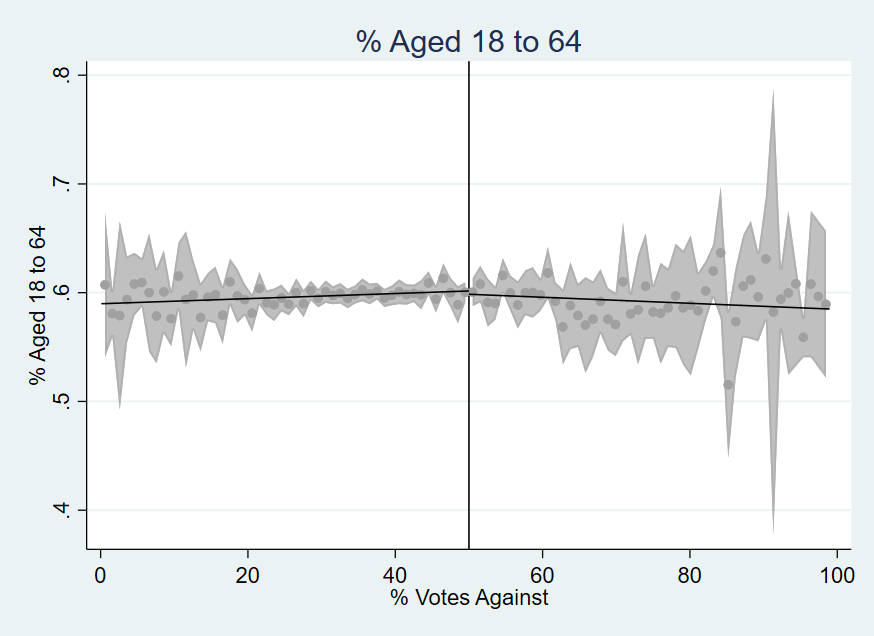
\includegraphics[width=\textwidth,keepaspectratio]{images/cov_smoothness_pct18to64.png}
        \caption*{Pct 18 to 64}
        \label{fig:pct18to64_sm}
    \end{minipage}
    \hfill
    \begin{minipage}[b]{0.40\textwidth}
        \centering
        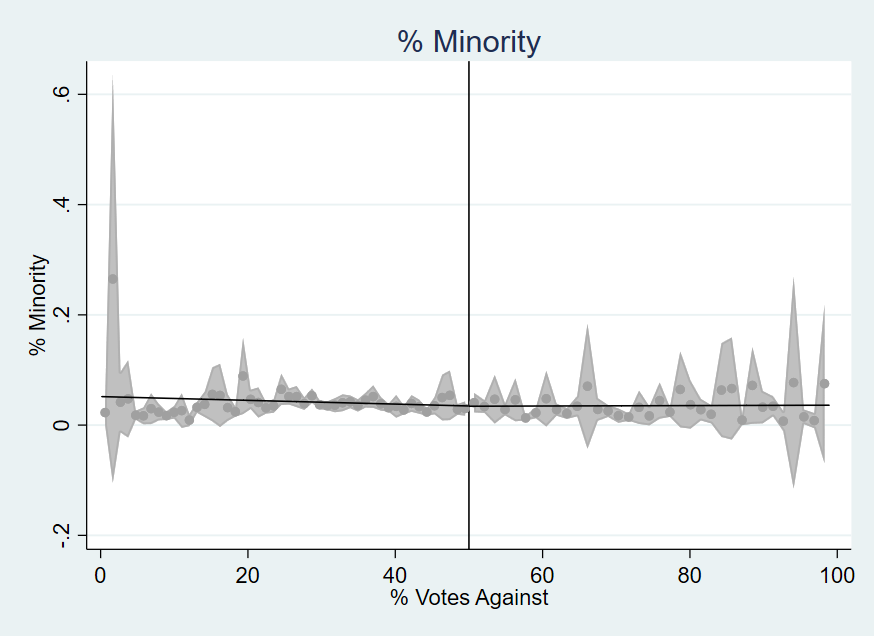
\includegraphics[width=\textwidth,keepaspectratio]{images/cov_smoothness_pctmin.png}
        \caption*{Pct Minority}
        \label{fig:pctmin_sm}
    \end{minipage}
    
    \caption{Covariate Discontinuity Plots - Part 2}
    \label{fig:rd_cov_smoothness_2}
\end{figure}


\clearpage


\section{Additional Information} \label{sec:appxc}

% \subsection{A Case Study of Roads in Waynesville OH: Serial Cutter of Road Maintenance Tax Levies}
\subsection{More Details on Predicting Road Quality} \label{sec:appxc1}

Coming very soon.

\subsection{Road tax levies vs. Other types of levies}

\begin{table}[ht!]
    \centering
    \caption{Correlation of Road Tax Levy Referenda Results with Other Types of Levies}
    \begin{tabular}{lcccccc}
    \toprule
    & Police & Fire & Current Expenses & Recreational & School \\
    \midrule
    Estimate & 0.248 & 0.053 & 0.388*** & 0.015 & -0.024 \\
    & (0.153) & (0.043) & (0.099) & (0.317) & (0.092) \\
    \bottomrule
    \end{tabular}
    \begin{minipage}{\textwidth}
    \footnotesize
    \textit{Notes:} This table presents coefficients from regressions correlating road tax levy referendum outcomes with outcomes for other types of levies (police, fire, current expenses, recreational, school). Standard errors are reported in parentheses. The coefficient for "Current Expenses" is statistically significant at the 1\% level (***). All regression control for year and neighborhood fixed effects, as well as neighborhood characteristics. The school levy analysis is conducted at the county level, while all other analyses are at the county subdivisions level. Statistical significance levels are indicated as follows: *** $p<0.01$, ** $p<0.05$, * $p<0.1$.
    \end{minipage}
\end{table}

% \begin{figure}[ht]
%     \centering
%     \begin{minipage}[b]{0.48\textwidth}
%         \centering
%         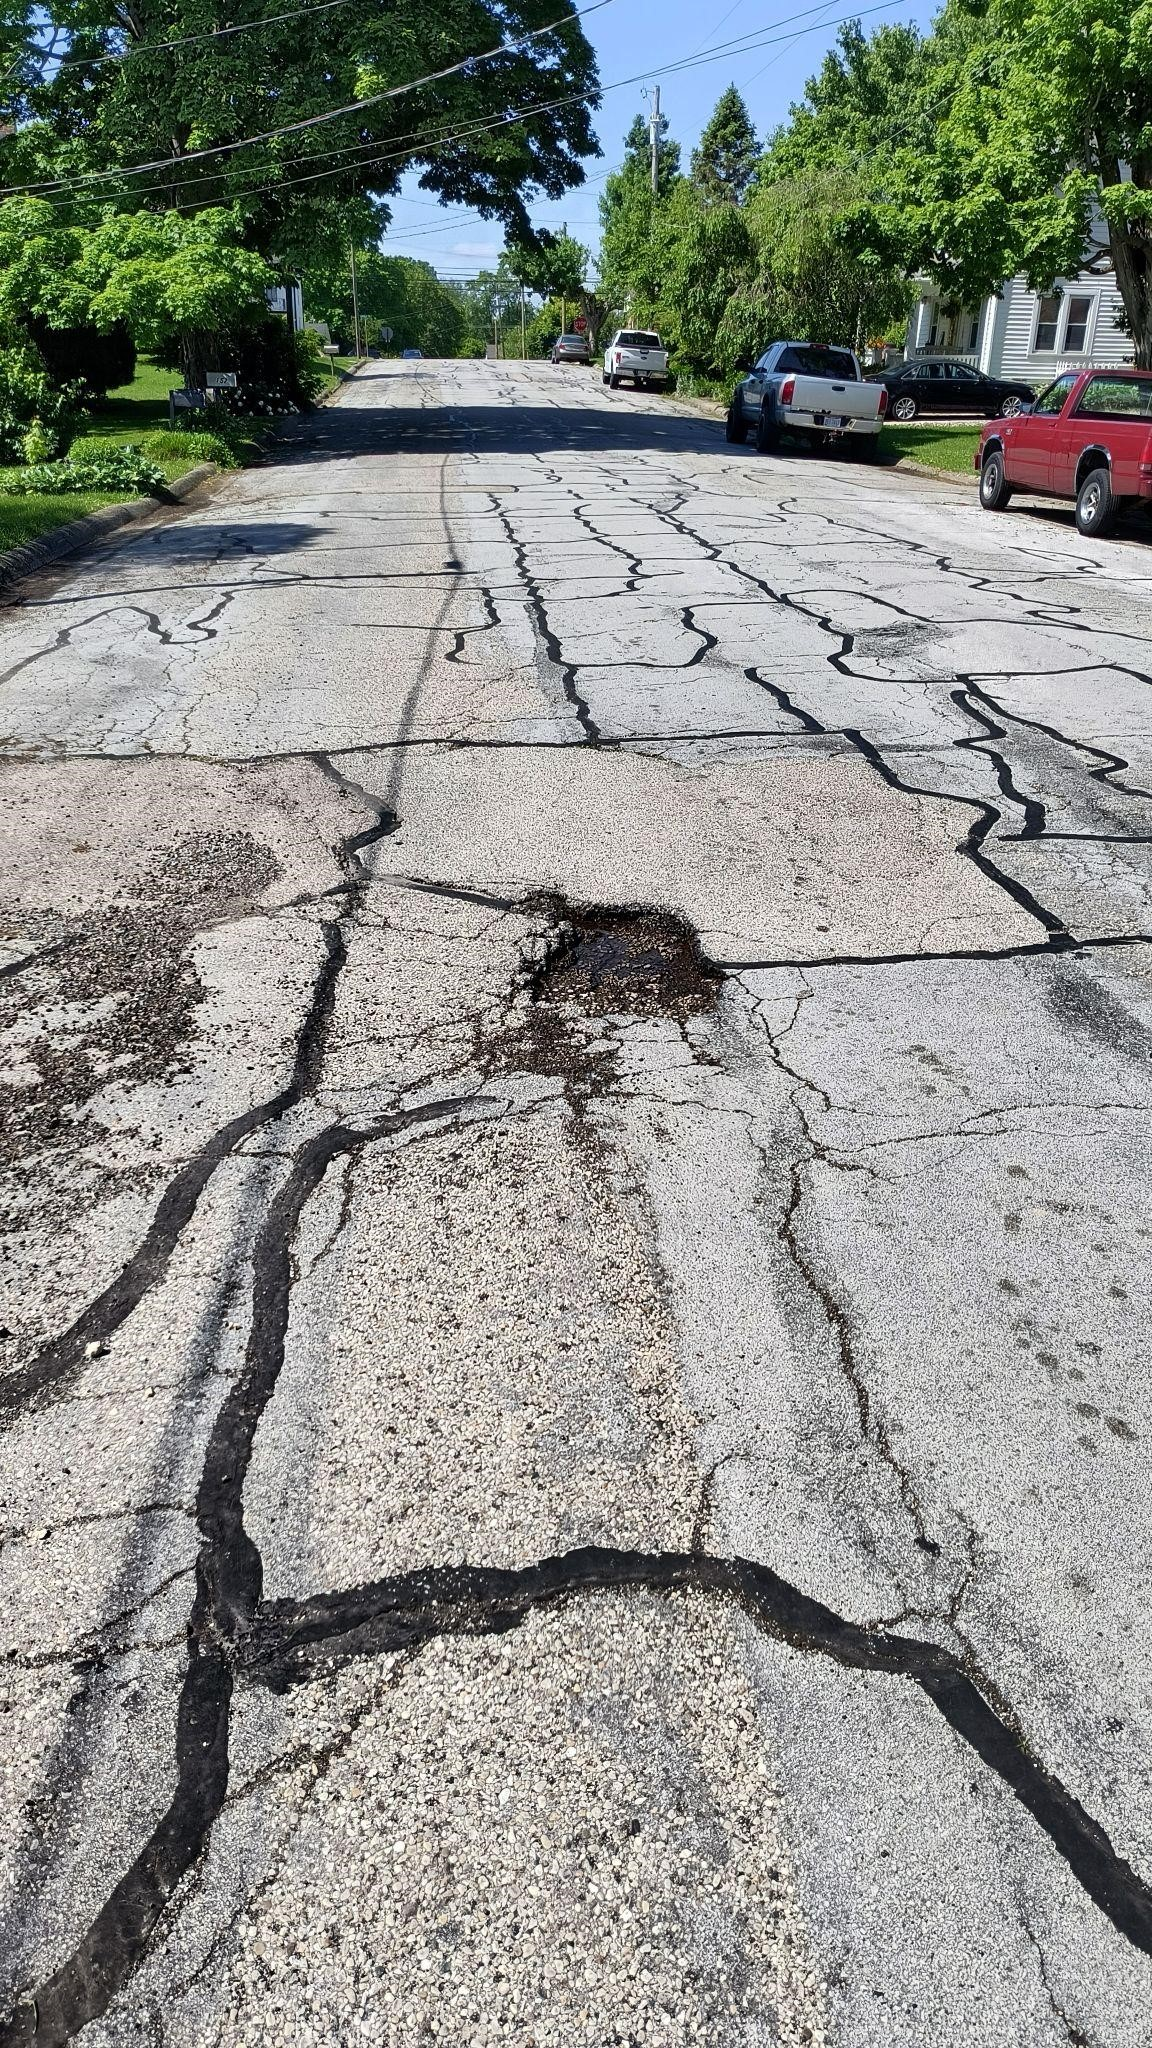
\includegraphics[width=0.75\textwidth,keepaspectratio]{images/waynesville_oh_1.png}
%         \caption*{Waynesville Road Image 1}
%         \label{fig:w_oh_1}
%     \end{minipage}
%     \hfill
%     \begin{minipage}[b]{0.48\textwidth}
%         \centering
%         \includegraphics[width=0.75\textwidth,keepaspectratio]{images/waynesville_oh_2.png}
%         \caption*{Waynesville Road Image 2}
%         \label{fig:w_oh_2}
%     \end{minipage}

%     \vspace{1em}

%     \begin{minipage}[b]{0.48\textwidth}
%         \centering
%         \includegraphics[width=0.75\textwidth,keepaspectratio]{images/waynesville_oh_3.png}
%         \caption*{Waynesville Road Image 3}
%         \label{fig:w_oh_3}
%     \end{minipage}

%     \caption{Roads in Waynesville: Case Study}
%     \label{fig:rd_waynesville}
% \end{figure}

% \section{More Details on Predicting Road Quality} \label{sec:appxd}
